\documentclass[conference]{IEEEtran}
\IEEEoverridecommandlockouts

\usepackage{cite}
\usepackage[pdftex]{graphicx}
\usepackage{cite}
\usepackage{amsmath,amssymb,amsfonts}
\usepackage{algorithmic}
\usepackage{graphicx}
\usepackage{textcomp}
\usepackage{xcolor}
\def\BibTeX{{\rm B\kern-.05em{\sc i\kern-.025em b}\kern-.08em
    T\kern-.1667em\lower.7ex\hbox{E}\kern-.125emX}}

\usepackage{url}

% correct bad hyphenation here
\hyphenation{op-tical net-works semi-conduc-tor}

% Regler ti skrivning: 
% 1. Altid nutid
% 2. Brug 1. persons flertal stedord (We/us/our/ours)
% 3. Skriv formelt og uden sammentrækninger (don't do this) 
% 

\begin{document}

\title{Telemetry Module for Solar Vehicle}

\author{\IEEEauthorblockN{Victor Alexander Hansen s194027, Steffan Martin Kunoy s194006, Tjark Petersen, s186083}
\IEEEauthorblockA{\textit{Department of Electrical Engineering} \\
\textit{Technical Uniservity of Denmark}\\
Kgs. Lyngby, Denmark \\
31015 Introductory project - electrotechnology\\
s194027@student.dtu.dk, s194006@student.dtu.dk, s186083@student.dtu.dk}}
%\author{Victor Alexander Hansen, Steffan Martin Kunoy, Tjark Petersen}

\maketitle

% As a general rule, do not put math, special symbols or citations
% in the abstract or keywords.
\begin{abstract}
Abstract
\end{abstract}

% Note that keywords are not normally used for peerreview papers.
\begin{IEEEkeywords}
ROAST, telemetry, CAN
\end{IEEEkeywords}



\section{Introduction}

\IEEEPARstart{I}{n} 2023, DTU Roadrunners Solar Team, abbreviated ROAST, is set to participate in the Bridgestone World Solar Challenge, a race spanning over 3000 km across Australia from Darwin in Northern Territory to Adelaide in South Australia. The solar car has limited opportunities for recharging during the race, so the main energy source during the race will be the sun. To this end, solar panels will cover the car, however, the solar car is only allowed to have a maximum of 4 square meters of solar panels. This emphasizes the need to create an energy-efficient solar car to win the race \cite{wsc}.\\
Throughout the race the solar car will be monitored by a support vehicle, which can monitor the car's condition and should be able to issue commands to the solar car's internal systems. This is a crucial function as the solar car will be navigating Australia's busy highways, where the heat and tire pressure may cause a detriment to the vehicle. The support car will therefore be able to analyze and react to the data stream being transmitted from the solar car, even when the driver is preoccupied by driving the car and navigating traffic. \\
The main function of the telemetry module is to read data from the solar car's on-board CAN (Controller Area Network) bus and transmit it via an RF-transceiver to the support vehicle, while simultaneously logging data in a local storage acting as a "black box". The support vehicle is equipped with a similar module such that the support crew can react to the data manually or automatically by sending commands back to the CAN bus. As a consequence, the telemetry module plays a vital role in the communication between both vehicles, considering that the distance between them may be up to 1 km depending on traffic conditions.\\
Therefore, the telemetry module must both serve the purpose of fulfilling the necessary specifications for communication, while also being as energy-efficient as possible. This project will mainly focus on the former, that is, ensuring that the module meets the specifications with a solid solution.

\subsection{Problem Statement}
Remote sensing of data from the solar car will give the ROAST team a competitive advantage as the support vehicle will be able to take on a more active role in managing and optimising the car's performance. This will ease the burden on the driver and leverage the expertise of the supporting crew. For these reasons we have chosen to focus our project on the following points:
\begin{itemize}
    \item How can we design a module that can read and write sensor data and commands from a CAN bus network? 
    \item How can CAN data be transmitted securely over a distance of up to one kilometer?
    \item How does the support-car module process data upon receiving it from the solar car?
    \item What is the best method for storing data locally (black box) while being accessible at a later time?
    \item How can the CAN data be made accessible in the support vehicle for further processing e.g. in Matlab?
\end{itemize}

\section{Methodology}
The project methodology has largely consisted of making a preliminary design to be completed in a series of design sprints. At first a detailed specification was drafted which then served as a reevaluation tool and an overall guidance each time a sprint was completed and when the goal for the next sprint had to be selected. Using the specification, we made a prototype setup of the hardware on breadboards as our first sprint. The following sprints would then mostly have software development objectives, such as achieving a first transmission and receiving of data. Finally, a last hardware sprint was conducted where we soldered our hardware to a perf board.\\
During the development of the software functions, we also verified and validated our code design. In verification the code and its functionality was discussed. To validate our code we made unit tests that test the actual behaviour of our code against the intended behaviour.\\
During the software development phase, we attempted to make our debugging more efficient with the use of a debugger. However, this proved quite troublesome, as the Teensy 3.6 board does not have an on-board debugger and in general is not very suited for debuggers. If we had insisted on using a debugger such as st-link, we would have had to hold or solder wires to the debug ports on the Teensy board's backside, which would complicate our prototype setup. Therefore, we decided not to spent more time on finding a debugger solution. This was a clear setback, as debugging could only be conducted by sending text over the serial connection.
\section{Design}
Overall specification?

Block diagram

\subsection{Components}

\subsection{Software Stack}

In this section the main software tools and libraries used throughout the project are introduced.

\subsubsection{PlatformIO}
The Teensy micro-processor line-up is integrated into the Arduino framework and implements as such the Arduino standard API. As a cross-platform build tool, PlatformIO is a more potent alternative to the standard Arduino IDE including more advanced features such as a static code analyzer and even a remote unit testing framework.

\subsubsection{ChibiOS}
An open-source RTOS for embedded systems including Teensy. It supports threads, semaphores, data-sharing and timers and more to ease the scheduling of different tasks by the program kernel. 

\subsubsection{Other Libraries}

\subsection{CAN} % Victor
The CAN network in the solar car enables the micro-controllers at each electrical unit in the car to send and receive data without a host computer. This is possible with the special structure of the CAN message.\\
\begin{figure}[h]
    %\centering
    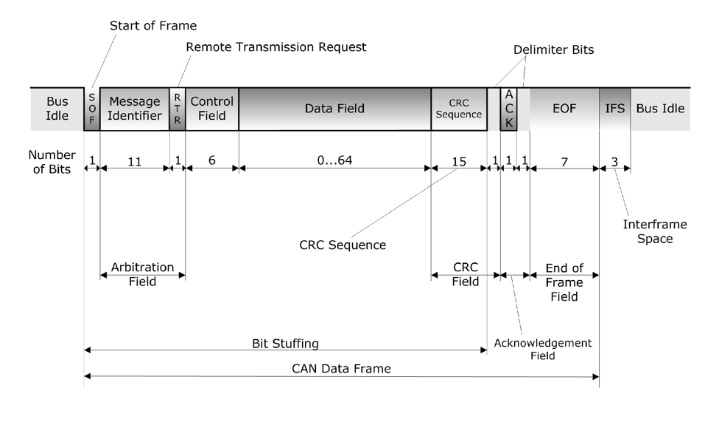
\includegraphics[scale=0.35]{documentation/images/detailed-can-data-frame-architecture.jpg}
    \caption{Structure of a CAN frame}
    \label{fig:CANframe}
\end{figure}\\
The frame uses an identifier to tell which messages goes to which unit. When two messages tries to access the bus, the one with the highest priority, lowest ID, will be granted access to the bus, while the other message has to wait. After the ID comes the RTR bit which determines whether the frame is set to be at sent or received by the node. The control field, sometimes called DLC, tells the amount of bytes used in the following frame field with actual data. The rest of the fields in fig. \ref{fig:CANframe} is not important concerning the nodes ability to communicate across the CAN network.\\
The CAN bus itself is two twisted wires, CAN High and CAN Low. These control the bits in the CAN message by setting a dominant and recessive voltage, which corresponds to a 0 and 1 respectively. A 1 is seen when the voltage in both wires is 2.5V while a 0 is seen when the CAN High wire is driven by 3.5V and the CAN Low wire is driven at 2.5V. 
\subsection{RF module} % Steffan 
The nRF24L01+ LoRa RF module is used to provide two-way communication between the solar car and support vehicle. It satisfies all the communications requirements a range exceeding 1000 m with and transmission rate of up to 2 Mbit/s. In addition, comprehensive driver libraries are provided, allowing us to raise the abstraction of our transmission protocol. \\


\subsection{Message protocol}
The nRF24L01 module uses the Enhanced Shockburst packet structure to transmit messages over the 2.4 GHz ISM band. The package 

\begin{figure}
    \centering
    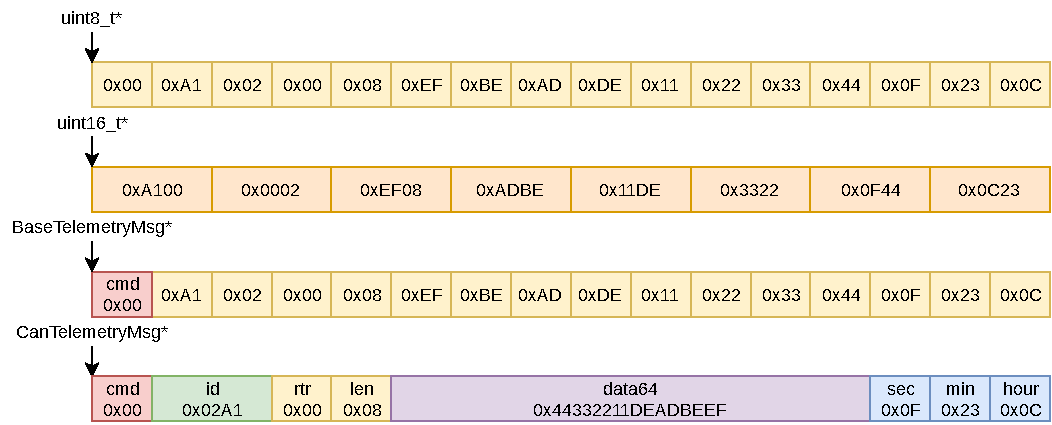
\includegraphics[width=\linewidth]{documentation/images/MessageTypes.pdf}
    \caption{The }
    \label{fig:my_label}
\end{figure}

\section{Implementation}

\subsection{Solar Car} 
\subsubsection{Black Box} % tjark
\subsubsection{CAN transceiver}
\subsection{Support Vehicle}
\subsubsection{GUI} % tjark
\subsubsection{RF transceiver}

\section{Verification and validation} % Victor
As mentioned in the methodology section, we spent time thoroughly verifying and validating our code design. We undertook the software verification after finishing the prototype and software coding, reviewing the naming, functionality and commenting the code accordingly.\\
We performed software validation as we went along with the software coding, to make sure that the actual behaviour of the code was as the expected behaviour. This was done through the testing environment in PlatformIO. We used this to validate our code design with unit tests, testing both edge cases and random cases. We chose only to validate the code and functions we made ourselves, and not those that was imported from external libraries.\\
Doing this provided us a test bench for our project, which greatly improved the credibility of our work, proving that our design works in general cases and not just the case we represent in our report.

\section{Discussion}

\section{Conclusion}
The conclusion goes here.


% use section* for acknowledgment
\section*{Acknowledgment}


The authors would like to thank Martin Schoeberl and Christian Kampp Kruse for their mentoring and assistance throughout the project. The authors would also like to thank Claus from the department of Mechanical Engineering at DTU.

\bibliographystyle{IEEEtran}
\bibliography{IEEEabrv,../bib/paper}

\section{References}
\begingroup
\renewcommand{\section}[2]{}%
%\renewcommand{\chapter}[2]{}% for other classes
\begin{thebibliography}{}
\bibitem{wsc}
Bridgestone World Solar Challenge, 
URL: https://worldsolarchallenge.org/
\bibitem{ROAST}
Reports and source files provided by DTU ROAST
\bibitem{teensy}
Teensy microcontroller,
URL: https://www.pjrc.com/teensy/
\bibitem{C++}
Website for learning C++
https://www.learn-cpp.org/
\bibitem{Aunit}
Documentation,
https://www.arduino.cc/reference/en/libraries/aunit/
\end{thebibliography}
\endgroup


\end{document}
